\documentclass{article}
\usepackage[utf8]{inputenc}
\usepackage{multicol}
\usepackage[style=numeric,backend=bibtex]{biblatex}
\usepackage{graphicx}
\usepackage{caption}

\addbibresource{refsKami.bib}

\title{Machine Madness}
\author{
  Amogh Param\\
  704434779\\
  \texttt{aparam@cs.ucla.edu}
  \and
  Sravani Kamisetty\\
  304414410\\
  \texttt{skamisetty@cs.ucla.edu}
}
\date{December 2015}

\begin{document}
    \maketitle
    
    \begin{multicols}{2}
    \section*{Abstract}  
	March Madness is the NCAA Men’s Division I Basketball Championship tournament that happens every March. The tournament is organized by the National Collegiate Athletic Association (NCAA). It has 64 tournament matches. The aim of this project is to come up with a good machine learning based model has the best classification accuracy in predicting the march madness bracket.
   
    \section{Introduction}
    Since 1939, the best colleges and universities across the United States have participated in a yearly tournament called the NCAA Men’s Basketball Championship. This basketball tournament has become one of the most popular and famous sporting tournaments in the United States. Millions of people around the country participate in contests in which the participants make their best guesses on who will win each game throughout the tournament. These types of contests have become so popular that more than 11 million brackets were filled out on ESPN.com in 2014. One billion dollars was even being rewarded to anyone who achieved a ”perfect bracket” (guessed every game correctly). Every game is unpredictable, and the teams that are supposedly the ”better team” sometimes end up losing. This is called an upset in basketball lingo, and happens regularly throughout the tournament. Because of these upsets, it can be difficult to correctly guess the winner of each game. The tournament can be so unpredictable that the time period over which the tournament runs has been termed March Madness. Since there are 64 games played in the NCAA tournament, it is nearly impossible to predict a perfect bracket. High Point Enterprise, a morning paper from North Carolina, stated that ”you have a much greater chance of winning the lottery, shooting a hole-in-one in golf or being struck by lightning”. They estimated that the chances of predicting a perfect bracket are 1 in 9.2 quintillion. It became clear that developing a model that provided perfect win/loss classification was unrealistic, so instead we focused on improving the prediction accuracy of individual games. The problem at hand is not classification of individual teams, but rather predicting the outcome of a match between any two teams. 
    
    \subsection{Objectives}
    Our goal was to identify key factors in predicting NCAA tournament wins and to find a
model that would perform well in the Kaggle competition.
The Kaggle competition had two stages:
\begin{list}{•}{•}
\item Predict outcomes of the 2016 NCAA Tournament
\end{list}
    For each stage we submitted a list $\hat{y}$ of probabilities (values between 0 and 1) that each team in the tournament would defeat every other team in the tournament, regardless of whether this match-up actually occurs. For this year, this was m = 2278 predictions 2. We were judged based on the log-loss L(y|$\hat{y}$), or the predictive binomial deviance, of the games that actually occurred.
    \linebreak 
    \linebreak 
    $L(y|\hat{y}) = -1/n * \sum_{i=1}^{n}[y_i.log(\hat{y_i} + (1-y_i). log(1-\hat{y_i}))]$ where n is the actual number of games played in the tournament (67), $y_i$ is the actual binary outcome of each game, and $\hat{y_i}$ is the corresponding submitted probability. If the opponents in game i are teams A and B, then $\hat{y_i}(A,B)$ is the predicted probability that team A beats team B, and $\hat{y_i}(B,A)=1-\hat{y_i}(A,B)$
   \linebreak
   \linebreak
   The goal is to find a set of predictions $\hat{y}$ that minimizes L(y|$\hat{y}$) for the unknown outcome vector y. This scoring method heavily penalizes being simultaneously confident and wrong. If we say Team A will beat Team B with probability 1 and Team B wins, then our log-loss is infinite (although Kaggle bounded the log-loss function to avoid infinite scores). At the same time, it is important to balance between being too conservative and too confident. If we are too conservative (e.g. $\hat{y} \approx 0.5)$, then we will never accrue points, but if we are too confident, we make ourselves vulnerable to huge losses.\cite{1}

	\section{Challenges}
	\subsection{Upsets}
	Every game is unpredictable, and the teams that are supposedly the ”better team” sometimes end up losing. This
is called an upset in basketball lingo, and happens regularly throughout the tournament. Because of these upsets, it can be difficult to correctly guess the winner of each game. The tournament can be so unpredictable.\cite{2}

	\subsection{Chance of predicting a perfect bracket}
	Since there are 64 games played in the NCAA tournament,
the odds of forecasting a perfect bracket are astronomical. Each game win/lose has a probability of 1/2. The complexity of the bracke prediction is 1/2*1/2..1/2 (63 times) which is 1 in $~approx$ 9.2 quintillion channce. This is lower than the chance of winning a lottery.

	\subsection{Unpredictable events}
	There are multiple events that happen during a match that cannot be predicted. The best example being injury of a key player. A new player being added to a team is one other such example. Playing at home ground vs playing else where sometimes also affects the outcome of the match.
	
	\subsection{Team Dynamics}
	The dynamics of a team change yearly. New players could be added, older key players could be removed. This makes it difficult to compare the performance of a new team to a old team as the logistics and features of an older team do not represent the newer team accurately. 
	
	\section{Data}
	The main source of Data is Kaggle. The data is made availabe as a bunch of .csv files. Kaggle provides regular season wins, losses, point differences, dates, and game locations (home/away) as well as tournament wins, losses, point differences, seeds, and dates of games. This data comes from the sesonal and tournament mactches for the years 2005-2015. \cite{1}. The other important source of data is player level statistics from ESPN.
	\linebreak 
	The data provided by Kaggle can be broadly classified into team statistics and match statistics \cite{1}
	\subsection{Match Statistics}
	This data fields identifying the different seasons included in the historical data, along with certain season-level properties are:

\begin{list}{Field}{}
\item 
"season" - indicates the year in which thetournament was played
\item
"dayzero" - tells you the date corresponding to daynum=0 during that season. 
\item
"region W/X/Y/Z" - by convention, the four regions in the final tournament are always named W, X, Y, and Z.
\end{list}

	The game by game results are represented by the following data fields:
\begin{list}{Field}{}
\item
wteam" - this identifies the id number of the team that won the game
\item
"wscore" - this identifies the number of points scored by the winning team.
\item
"lteam" - this identifies the id number of the team that lost the game.
\item
"lscore" - this identifies the number of points scored by the losing team.
\item
"numot" - this indicates the number of overtime periods in the game, an integer 0 or higher.
\item
"wloc" - this identifies the "location" of the winning team. If the winning team was the home team, this value will be "H".
\item
"wfgm" - field goals made
\item
"wfga" - field goals attempted
\item
"wfgm3" - three pointers made
\item
"wfga3" - three pointers attempted
\item
"wftm" - free throws made
\item
"wfta" - free throws attempted
\item
"wor" - offensive rebounds
\item
"wdr" - defensive rebounds
\item
"wast" - assists
\item
"wto" - turnovers
\item
"wstl" - steals
\item
"wblk" - blocks
\item
"wpf" - personal fouls
\item
"seed" - this is a 3/4-character identifier of the seed, where the first character is either W, X, Y, or Z (identifying the region the team was in) and the next two digits (either 01, 02, ..., 15, or 16) tells you the seed within the region.
\item
"slot" - this uniquely identifies one of the tournament games. For play-in games, it is a three-character string identifying the seed fulfilled by the winning team, such as W16 or Z13. For regular tournament games, it is a four-character string, where the first two characters tell you which round the game is (R1, R2, R3, R4, R5, or R6) and the second two characters tell you the expected seed of the favored team.
\item
"strongseed" - this indicates the expected stronger-seeded team that plays in this game.
\item
"weakseed" - this indicates the expected weaker-seeded team that plays in this game, assuming all favored teams have won so far.
\end{list}
	
	\subsection{Team Statistics}
	The data provided by Kaggle also has certain statistics that describe the team itself. This represents a cumulative performance of a team for the last 10 years. Some of the most important team statistics are:
	\begin{list}{•}{•}
\item
	Two point field goals made 
\item
Three point attempts
\item
Assists per game
\item
Average scoring margin
\item
Blocks for season
\item
Defensive rating
\item
Field goal percentage
\item
Total free throw attempts
	\end{list}
	\subsection{Scale of the Data}
	Kaggle provides data from the NCAA seaons and tournaments between 2005 and 2015. The statistics below give an idea about the scale of the dataset.	
\begin{list}{•}
\item
Number of seasons: 10 seasons
\item
Number of tournaments: 10 tournaments
\item
Number of matches in each season ~ 5000
\item
Number of matches in each tournament ~ 64
\item
Total number of matches in the training set ~ 50,640
\item
Total number of matches in testing set : 64
\item
Total number of columns in the training set/testing set ~ numeber of data fields or features $\approx$ 40
\end{list}

	\section{Features}
	As described in the section 3.a and 3.2 the data provided by Kaggle has a lot statistics compiled for every
basketball game, so it was difficult to decide which ones to use. Hence we used all the feautures initially to construct a training set. Dimensionality reduction was then performed on the training set to pick the most important features.

	\subsection{Feature Representation}
	The final goal of the Kaggle March Madnness competition is bracket prediction. This means that we have to predict the outcome of the 64 tournament mactches that happen in NCAA 2016. The best bet to do this is if we have a training set that represents the matches and labels that represent the outcomes of these matches. All the data statistics discussed in the section 3.1 and 3.2 can be represented in 2 ways to achieve this goal
\begin{list}{•}	
\item
	Vector of difference: Each match is represented by the vector of difference between the induvidual statistics of the 2 teams. This essentially means that the training vector \linebreak 
	$X  =  mod(Statistics of Team A $
	\linebreak	
	$- Statistics of Team B)$. 
	\linebreak
	The result or the label vector Y is represented by 0/1. The result is 1 if Team A beats Team B 
and 0 if Team B beats Team A.
	
	\item 
	Concatenated Vector of both the team statistics: In this representation the statistics of a match is represented by keeping both Team A and Team B statistics in the vecotor next to each other. Hence the training vector 		\linebreak
	$X = [Statistics of Team A , $
	\linebreak	
	$Statistics of Team B]$.
	\linebreak
	The result or the label set representation is same as the previous case.
	\end{list}
	
	\subsection{Additional Features}
	A few additional features were computed separately and added to the training set for every match. These additional features are obtained by applying algorithms to already existing team and match statistics and considering the value given by the algorithm as a feature itself. 
\subsubsection{Team Rank}
A method similar to PageRank algorithm called the GEM method was applied to the NCAA dataset \cite{3}.  The margin of victory $(v1-v2)$ is used as the weight the “link” between two football teams, where v1 and v2 are the teams’ scores against each other. Then the process same as PageRank is followed to make it row stochastic. This will help us obtain the final ranking. Below is an example of the team Rank calculation.
	
	\begin{center}
	  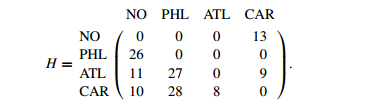
\includegraphics[height=15mm]{images/TeamRankMatrix.png}
	  \captionof{figure}{Team Rank Matrix}
	\end{center}
	This team rank matrix is represented as a graph.
	\begin{center}
	  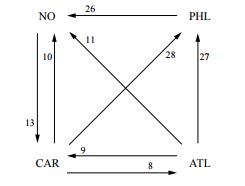
\includegraphics[height=25mm]{images/TeamRankGraph.png}
	  \captionof{figure}{Team Rank graph}
	\end{center}
Next, we continue to make it row stochastic and follow the PageRank algorithm to get the final ranking. We obtain (0.330 0.252 0.087 0.332) for the PageRank vector, which produces the ranking 1. CAR, 2. NO, 3. PHL, 4. ATL.

\subsubsection{Statistical Features}
	Statistical Features on Player Statistics: One more extra feature that was added to the training set at the lisr of top players that belong to every team. Only the top players that are playing a particular match are considered in the training set.

	\section{Architecture}
	The project can be divided into four important parts. They are data collection, feature extraction, machine learning model selection, predicitions step. Figure 3 is a pictorial representation of the architecture of the project. Programming languages python and the machine learning librares pandas, scikitlearn, tensorflow were used in the implementation of the project.	
	\begin{center}
	  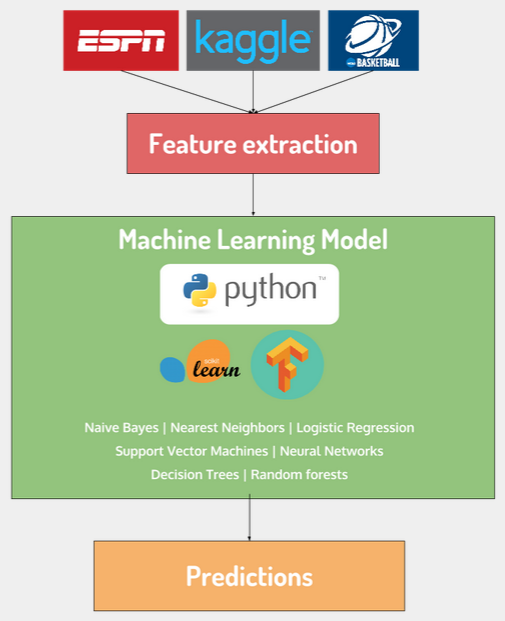
\includegraphics[height=110mm,width=50mm]{images/Architecture.png}
	  \captionof{figure}{Architecture}
	\end{center}
	
	\section{Dimensionality Reduction}
	\section{Machine learning Models}
	For reasons stated above in section 3, we wanted to use many different machine learning techniques and leverage them against one another so that we would gain the benefits from each and hopefully mitigate the weaknesses of each. We used Support Vector Machines, Random Forests, and Logistic Regression for the base level models.
	
	\subsection{Support Vector Machines}
	Each game in the training set X has a series of characteristics based on the difference in team statistics and a label yi (win or loss). These can be plotted in a p-dimensional Euclidean space. The support vector machine then finds the hyperplanes $w·X-b = 1$ and $w ·X = 0$ with the greatest distance between them that partitions the space such that wins and losses are separated (where w is the normal vector to the plane and $\left \| w \right \|/b$ is the offset of the hyperplane from the origin along w.)\cite{4}. Let the output of an SVM be $f(X)$. Then
	\linebreak
	\linebreak
$\hat{y_{i1}}(A,B)  = Pr(y_i = 1| f(X)) = 1/ 1+exp(Q * f(X) +V)$,
	\linebreak
	\linebreak
where Q and V are parameters chosen through maximum likelihood estimation from a training set made up of coordinates $(f(X)_i, y_i)$.\cite{4}

	\subsection{Decision Trees and Random Forests}
	Decision trees split a data set using a set of binary rules that make up the branches of the tree. Sets further down in the tree contain increasingly similar class labels. The objectives are to produce the purest sets possible and to be able to classify any object based on comparison of features to the rules in the tree. A random forest is a bootstrap of the decision tree. Like in the standard bootstrap method, the available training data can be resampled to build many different decision trees. Additionally, the random forest method takes a random subset of available predictors to build its new decision tree. By resampling both the cases and the input
variables, many decision trees are grown. Final classification decisions are made based on a majority rule of the many decision trees. Given a decision tree with height k, let $Pr(r_d)$ be the probability associated with node d on branch path r. Then the probability of success for a new case is:
	$y_i(A,B)=\prod_{d} Pr(r_d)$
	\linebreak
	\linebreak
For the random forest of m trees where $Pr(r_{(d, j)}
)$ is the probability associated with node
d on branch path r on decision tree j, the probability of success for a new case is:
	$y_i(A,B)=\sum_{j}\prod_{d} Pr(r_{(d,j)})$
	\subsection{Logistic Regression}
	 Logistic regression is a statistical method for analyzing a dataset in which there are one or more independent variables that determine an outcome. The outcome is measured with a dichotomous variable (in which there are only two possible outcomes). In logistic regression, the dependent variable is binary or dichotomous, i.e. it only contains data coded as 1 (TRUE, success) or 0 (FALSE, failure). In our case the dependent variable is the outcome of the match and independent variables are the features themselves. Logistic Regressio uses a logit function which measures the log odds of Team A winning a match against Team B: logit(p) = ln(p/(1-p)) where P is the probobality of A winning. 
	 
	 \subsection{Ensemble Model}
	 Ensemble methods are commonly used in classification problems. These methods allow predictions based on different models to be combined, often using a type of voting schema, to determine one final prediction. The benefit to using an ensemble method is that we can
leverage the information gleaned from different methods, combining the benefits from each method while hopefully negating or minimizing the flaws in each. Ensemble methods have been used to combine predictions from different machine learning techniques in order to increase stability and to more accurately classify test cases. The combination of methods can also reduce the variance of the predictions as they are less sensitive to irregularities in a training set.\cite{4}
	In order to ensure that our predictions were in (0,1), we fit a logistic regression model where each explanatory variable is a prediction from one machine learning technique, and the response is the binary outcome.
Our model takes the form:
\linebreak
\linebreak
$y_i(A,B) = 1/e^{-(\beta_0 + \beta_1y_1(A,B) +..\beta_3y_3(A,B) + \varepsilon )}$
where $y_1$ is from Support Vector machines, $y_2$ is from Random Forests and $y_3$ from Logistic Regression.

	\section{Performance and Evaluation}
	\subsection{Accuracy}
	
	\section{Conclusion}
	\section{FutureWork}	 
Even with large amounts of statistical information, there are some parts of a basketball game you simply cannot predict. Injuries cannot be forecast, and the mental state of players playing the game cannot be observed. However, these things can drastically affect the outcome of a basketball match. Perfect brackets will therefore continue to be impossible to calculate, no matter how much data is provided to the learning models.

\paragraph{}However, we believe that our classification accuracy can improve to above 75\% if the proper features are used in training. Vital statistical information we were unable to gather include the following:
\begin{list}{•}
\item
Venue of the match including the distance
\item
Importance of a match-up
\item
Average number of players who play consistently
\end{list}

All of this data is expected to play a role in how teams perform. However, this type of data was out of our scope to accumulate. Organizations with more access to this type of data will be able to study whether these features have a profound effect on the success of a basketball team. This research would also benefit greatly with more data. It is recommended that much more data be gathered to help avoid overfit. However, since basketball continually changes throughout the years, using data from more than ten years back is also useless. We would also recommend experimenting with using several feature reduction techniques together as opposed to using the reduction techniques one by one. This is something we did not explore as a part of the project.

\paragraph{} The overfitting problem can be solved by dividing the training set into 2 parts - training and evaluation. In this way the model can be built using training set, and fine tuned using evalution set. It can also be reduced by using some kind of regularisation in the model. It could L1 or L2 reguralisation depending on the machine learning model and parameters.
	\end{multicols} 
\end{document}
